\section{Complementary Techniques - Trace and Parameters Analysis as \mas support (\textcolor{blue}{All this section is new for TSE journal})}\label{sec:complementary}


%Our work, although closely related to previous studies, differs from them in several aspects.  First, our assessment is more comprehensive: instead of considering $102$ pairs of benign/malign apps, we execute our study considering \apps pairs of apps. We then investigate which characteristics of the malware samples in the large dataset explain the lower performance.
We expand our investigation by introducing two extensions to the \mas. The first extension leverages dynamic call graphs
to analyze the paths from entry points to calls made to sensitive APIs in both the original and repackaged versions of an application.
The second extension enhances the \mas by comparing the values of actual parameters used in the calls to sensitive APIs,
drawing inspiration from the work of Le et al.~\cite{le2018towards}. We conduct a series of experiments using our \cds,
employing three configurations of the \mas: (a) with the call-graph-based extension enabled,
(b) with the parameter-based extension enabled, and (c) with both extensions enabled.

\subsection{Call Graph Path Analysis}


Regarding call graph path analysis, we build the dynamic call graphs that characterize the execution of each version of the apps in our dataset. Our goal is to explore how many pairs of apps call the same set of sensitive APIs, though using different call traces. We hypothesize that differences in the traces might be used to complement the \mas for suspicious app identification. As such, here we execute the trace analysis for all app pairs of our \cds, and check if there are situations in which the basic version of the \mas was not able to correctly classify the malign version of an app as a repackaged, however it has a distinct execution trace. For detecting different trace, we performed an evaluation of the dynamic call graph of each app pair. Our procedure checks if there is some new node, representing a new sensitive API at malicious version, or a new edge($x$, $y$), where $x$ and $y$ indicates a method $x$ calling a sensitive method $y$. Figure~\ref{fig:callGraph} illustrates an example of benign and malicious call graphs.
At this example, although both app versions access the same set of sensitive resources, the
malicious version follows a different execution trace.




\begin{figure}[ht]
\centering
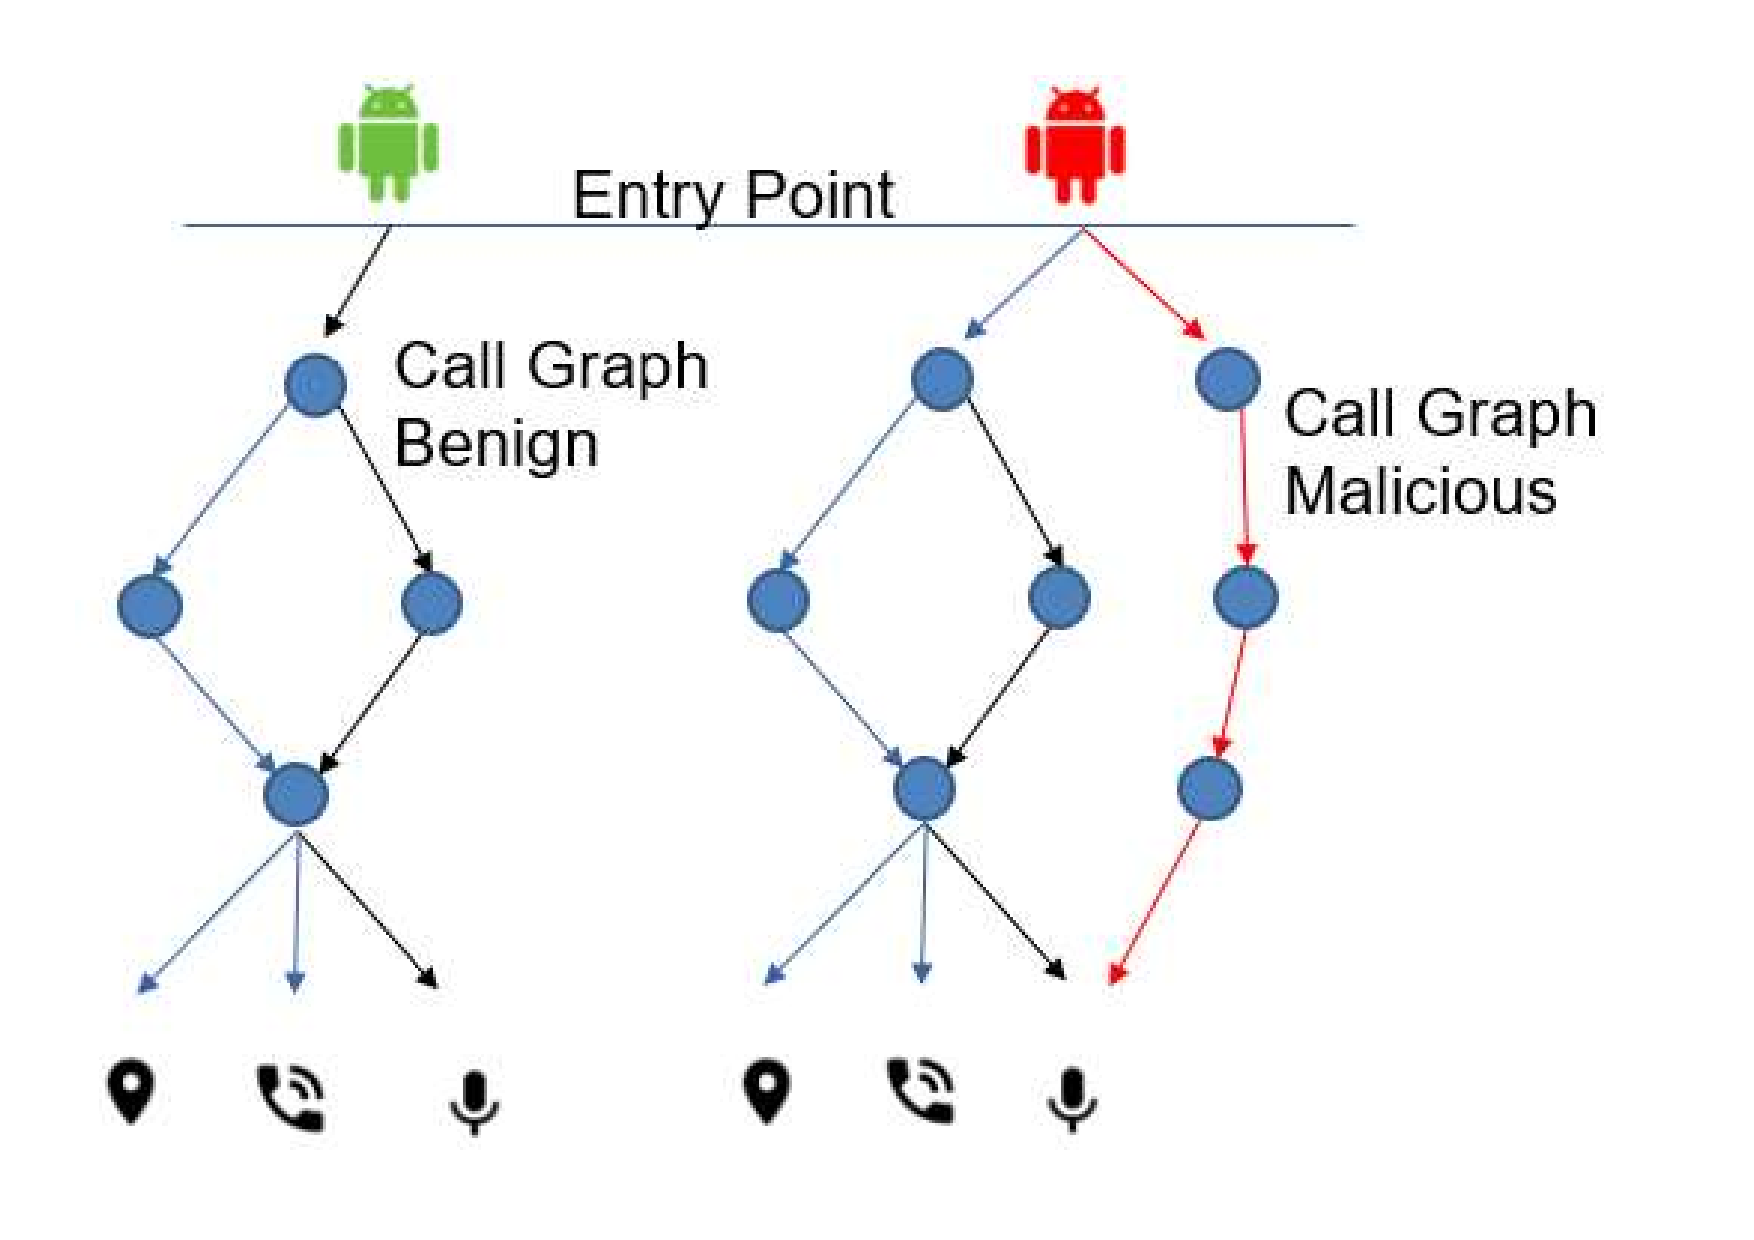
\includegraphics[scale=0.30]{images/maliciousCallGraph.pdf}
\caption{Illustrative example of the trace analysis. In this case, both versions call the same set of sensitive APIs. Nonetheless,
the traces between the entry point and the calls to sensitive APIs diverge.}
 \label{fig:callGraph}
\end{figure}


A real example, from our dataset, presents a trace injected in the malicious app version \textbf{[com.android.remotecontrolppt]} from original app (Figure~\ref{fig:maliciousTrace}). Here, the benign and malicious app versions access the same
sensitive method, \textit{getSubscriberid()}. This sensitive method returns the device's unique
subscriber ID, and requires the manifest file permission \texttt{READ\_PHONE\_STATE}, present in both app versions.
The original app accesses this method through two distinct traces (Trace 01 and Trace 02), which suggests an expected action from app user. However,
instead of the two original traces, the malicious version injected a third trace (Trace 03) containing as entry point a method that performs a stealth
computation on a background thread, \textit{doInBackground}, suggesting an action without user's awareness.

\begin{figure}
\centering
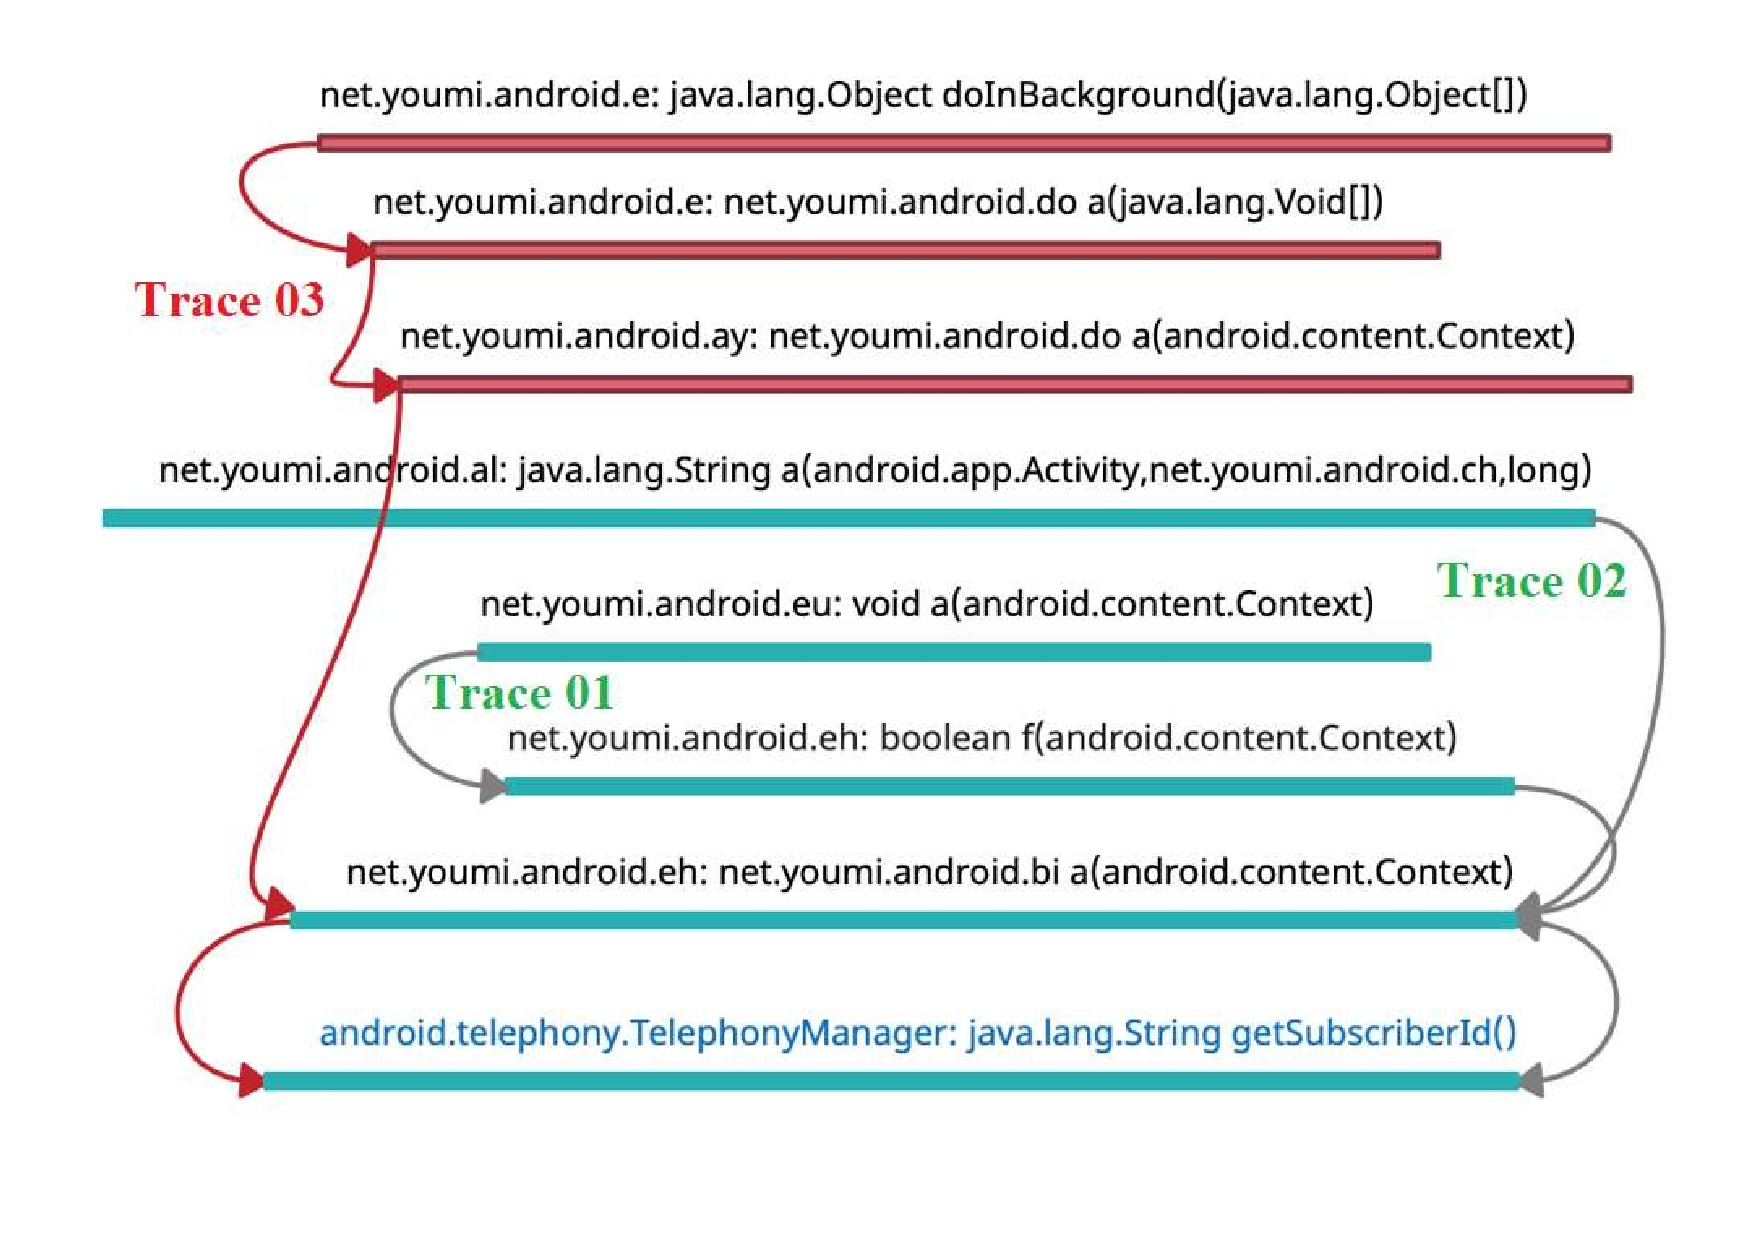
\includegraphics[scale=0.28]{images/maliciousTrace_example01.pdf}
\caption{Example of Malicious Trace.}
 \label{fig:maliciousTrace}
\end{figure}


The results of our investigation reveal that with trace analysis, we reduce the number of false negatives from $1,450$ to $1,327$, with the side effect of increasing the number of false positives from $252$ to $253$ (first and third row of Table~\ref{tab:accuracyParameter}). In the end, our trace analysis improved the accuracy ($F_1$) of \mas from $0.39$ to $0.45$, when compared with vanilla \mas.


\subsection{Parameter Analysis}

As described at~\cite{le2018towards}, malicious apps may require external data, like a remote server address to push an advertisement, or sink sensitive information to another location, different from the original, using SMS message for example. For this purpose, malicious apps may insert parameter in sensitive APIs, different from the original app. Thus, we also hypothesize that differences on the parameter (from both app versions), passed to the same sensitive APIS, may provides hints for suspicious repackaged apps. Figure~\ref{fig:parameterDiff} presents a real example of different parameters inserted at the same method, also extracted from our dataset \textbf{[com.nla.downloader]}. This example just use a \textit{java.net.URL} object to present a different advertising from the original app. Although not expressly harmful, repackaged apps may use objects from this \textit{Class} to download and run external files from a network in the infected system\cite{DBLP:journals/compsec/ObaidatSPP22}.

When we explore parameter analysis, we reduce the number of false negatives from $1450$ (vanilla \mas) to $1339$ samples, with the side effect of increasing the number of false positives from $252$ to $271$ (see the first and second row of Table~\ref{tab:accuracyParameter}).
In general, the accuracy ($F_1$) of the \mas using Parameter Analysis improves from 0.39 to 0.44 at \cds.



\begin{figure*}[t]
\centering
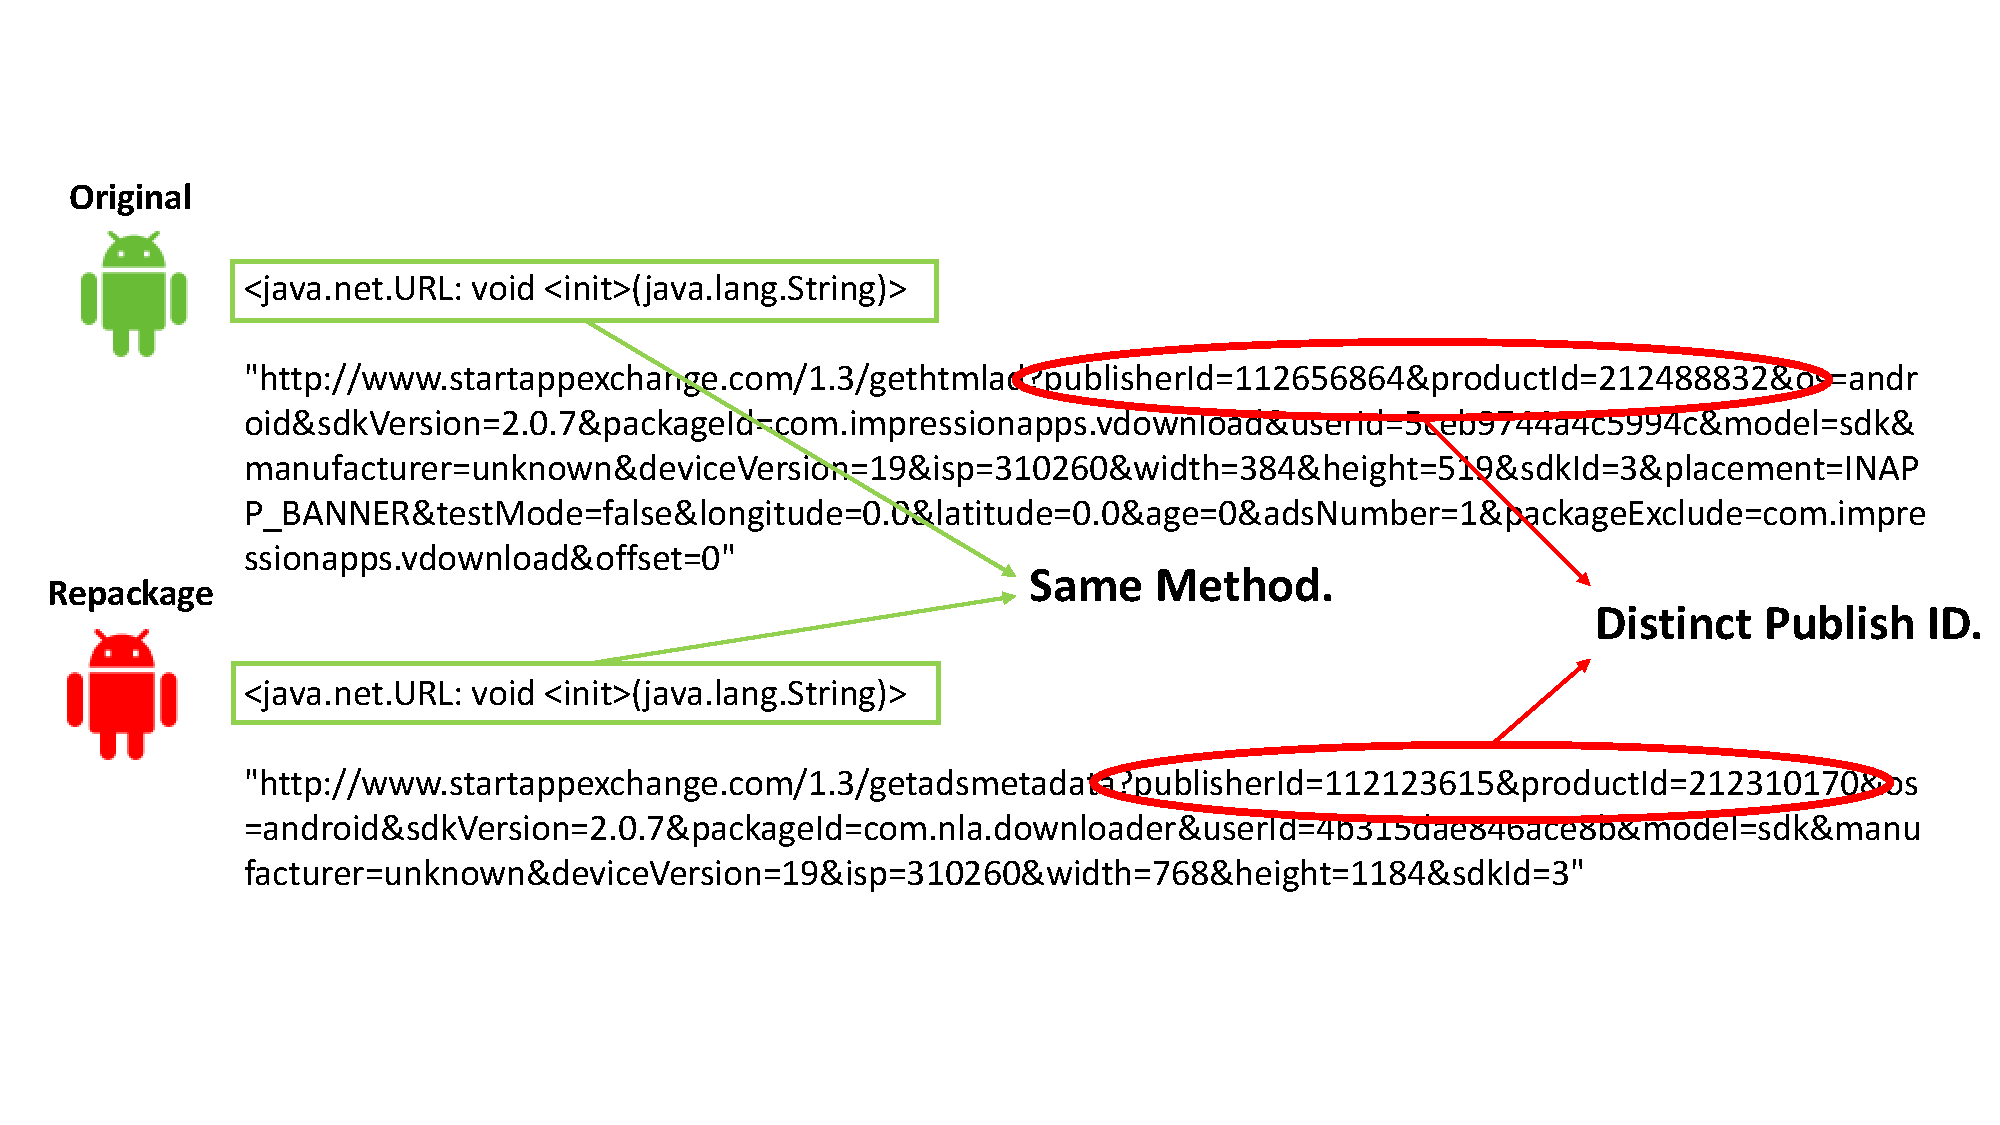
\includegraphics[scale=0.3]{images/parameterDiff.pdf}
\caption{Example of different parameters inserted at the same method.}
 \label{fig:parameterDiff}
\end{figure*}

\begin{table*}[ht]
  \caption{Accuracy of the \mas with aid of complementary techniques (3,211 app pairs).}
\centering{
  \begin{tabular}{lrrrrrr} \hline
    Dataset & TP   & FP  & FN  & Precision & Recall & $F_1$ \\ \hline
    
    %\mas + Traces  & \sds (102)   & 67   & 18  & 2   & 0.78      & 0.97   & 0.87  \\
    \cds \mas    & 545  & 252 & 1,450 & 0.68       & 0.27   & 0.39  \\
    \cds \mas + Trace     & 668  & 253 & 1,327 & 0.72       & 0.33   & 0.45  \\
    \cds \mas + Parameter     & 656  & 271 & 1,339 & 0.7       & 0.32   & 0.44  \\
    \cds \mas + Trace + Parameter     & 752  & 272 & 1,243 & 0.73       & 0.37   & 0.49  \\
    %\mas + Traces  & \cds (1203)   & 214  & 326 & 245 & 0.39      & 0.46   & 0.42  \\ 
    \hline
  \end{tabular}
  }
  \label{tab:accuracyParameter}
\end{table*}

\subsection{Combining trace and parameter analysis}

Additionally, we investigate if we could benefit from combining both techniques. When combining parameter and trace Analysis, we were able to detect $752$ (TP) of the repackaged apps ($23.41$\%). We reduce the number of FN from $1,450$ to $1,243$, however increasing the number of FP from $252$ to $272$. The combination of both techniques shows to be more effective than the vanilla \mas, or when we used just one of the techniques. In summary, the results of our studies reveal that the combination of both techniques present a ($F_1$) of $0.49$, as also reported in Table~\ref{tab:accuracyParameter}, improving the vanilla \mas.

\tb{5}{When combining both techniques, we reduces the number of false negatives (in comparison with the vanilla \mas), with the side effect of increasing the number of false positives. However, it improves the
overall accuracy ($F_1$) of \mas at malware detection, from 0.39\% to 0.49\% at \cds.} 
